\graphicspath{ {images/3_source_localization/} }
\chapter{Sound Source Localization}
\section{Physical background}
This section shows some underling fundamentals on which the following described theory is based on.
\todo{Schribe}

\section{Sound Source Localization Methods}
\acrfull{ssl} is a well researched area with many applications.
\cite{nat_skript}
The basic system can be brought into two categories, time based or power based methods.
\subsection{Power based SSL}
The idea of power based SSL is based of the known propagation properties of sound waves in air.
BlaBlaBla \todo{short text}
However for this method to work some properties of the sound source have to be known.
Additionally the sensors that measure the sound power levels have to be calibrated \dots

\subsection{Time Based SSL}
Another group of \acrshort*{ssl} is based on the time when the
signal is received by the microphones.
Given a source at a location $\bm{S} = (x_S,y_S)^T$ and $N$ microphones at locations
$\bm{M_n} = (x_n,y_n)^T$ the time it takes for a acoustic signal from the source to reach a microphone is
\begin{equation}
	t_n = \frac{\lVert \bm{S} - \bm{M_n}\rVert}{c}
	= \frac{\sqrt{\left(x_S - x_n\right) + \left(y_S - y_n\right)}}{c} .
\end{equation}
So if $t_n$ is known for a microphone, the location of the source can be limited to point on a circle
around $M_n$ with a radius of $t_n c$.
Given three or more microphones the intersection of these circles will show th location of the source.
However in many cases this approach is not realistic since $t_n$ is generally not know.
It would require some sort of a synchronization between the microphones and the sources.
\subsubsection{Near-Field}
The next time property that could be used is the \acrfull{tdoa} which between
two microphones $\bm{M_n}$ and $\bm{M_m}$ is defined as
\begin{equation}
	t_{n, m} = t_m - t_n = \frac{\lVert \bm{S} - \bm{M_m}\rVert - \lVert \bm{S} - \bm{M_n}\rVert}{c}.
\end{equation}
With this equation $\bm{S}$ can be interpreted as the set of points that lie on a hyperbola
which fixed points are the Microphones and the vertices are $c t_{n,m}$m apart.
To find the location of $\bm{S}$ a minimum of four microphones is now needed.
This approach works only if we can assume that the curvature of the incoming sound waves
at the microphones is big enough. Figure \ref{ssl:fig:near field} shows such a arrangement
which is generally known as the near-field scenario.
It is generally said, that the near-field assumption holds when the distance from the source
to the array isn't much greater than the size of the array.
In Figure \ref{ssl:fig:hyperbola} it can be seen how the resulting hyperbolas from the
\acrshort{tdoa} intersect at the point $\bm{S}$.


\begin{figure}[h]
	\centering
	\begin{subfigure}[b]{0.45\textwidth}
		\centering
		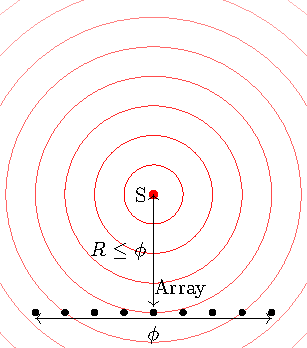
\includegraphics[width=\textwidth]{NearField.pdf}
		\caption{Acoustic model used for the near field \acrshort{ssl}.}
		\label{ssl:fig:near field}
	\end{subfigure}
	\hfill
	\begin{subfigure}[b]{0.45\textwidth}
		\centering
		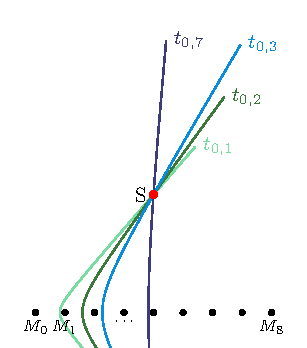
\includegraphics[width=\textwidth]{hyperbola.pdf}
		\caption{A selection of the hyperbolas resulting from the time-delays $t_{m,n}$.}
		\label{ssl:fig:hyperbola}
	\end{subfigure}
	\caption{Near field \acrshort{ssl} with a linear microphone Array.
		Since the microphones are distributed on a straight line a degree of freedom is lost and
		$\bm{S}$ mirrored at this line is also a possible solution.}
	\label{fig:three graphs}
\end{figure}

\subsubsection{Far-Field}
When the source is much further away than the size of the Array, as depicted
in Figure \ref{ssl:fig:far field}, the curvature of the sound wave at the array is negligible.
This is generally known as the far-field case.
Now the sound waves aren't modeled as spherical waves but rather as planar waves.
Given such a planar wave only the direction in which the source is placed can be determined with the TDOAs.

% Beamforming_general_S1110865703212038

\begin{figure}
	\centering
	%    \includegraphics[width=0.25\textwidth]{mesh}
	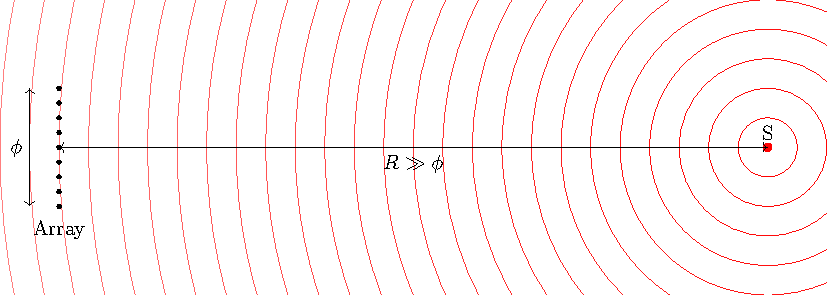
\includegraphics[]{FarField.pdf}
	\caption{Far-Field case. The Curvature of the sound-waves from S at the array
		is almost zero.}
	\label{ssl:fig:far field}
\end{figure}

\todo{Decission why this}
In this thesis the focus is set on the far-field case, due
\todo{literature}

\subsection{Direction of arrival estimation}
Lots of research has been made on how to estimate the \acrfull*{doa} of a source
with appropriate sensors.

\todo{brief lierature study}

In this thesis the focus was set on far-field techniques considering that the
goal is to detect drones which are usually several meters above ground.
%Constructing a microphone array 

\subsection{Beamforming}
Beamforming is a popular method for estimating the \acrshort{doa} of a signal.
Its fundamental principles are best shown in a visualization like
figure \ref{ssl:fig:beamforming1}.
For now the theory are shown in $\mathbb{R}^2$ and later expanded to $\mathbb{R}^3$.
The figure shows an source array where each source is emitting a
sine wave $x_n(t) = sin(\omega t + \phi_n)$ at a set point in time but each with a different
pre defined phase $\phi_n$.
By carefully selecting these phases the points where the waves positively
interfere form a beam.
Given this example with a narrow band signal, the signal at each source
can be written as
\begin{equation}
	x_n(t) = \Re(sin(\omega t) e^{j\omega \phi_n})
\end{equation}
and more generalized
\begin{equation}
	X(t) =
	\Re\left(
	sin(\omega t)
	\underbrace{\begin{pmatrix} e^{j\omega \phi_0} \\
			e^{j\omega \phi_1} \\
			\vdots             \\
			e^{j\omega \phi_{N-1}}
		\end{pmatrix}}_{W(\theta)}
	\right).
\end{equation}
The vector $W(\theta)$ is commonly known as the steering vector.

\begin{figure}
	\centering
	%    \includegraphics[width=0.25\textwidth]{mesh}
	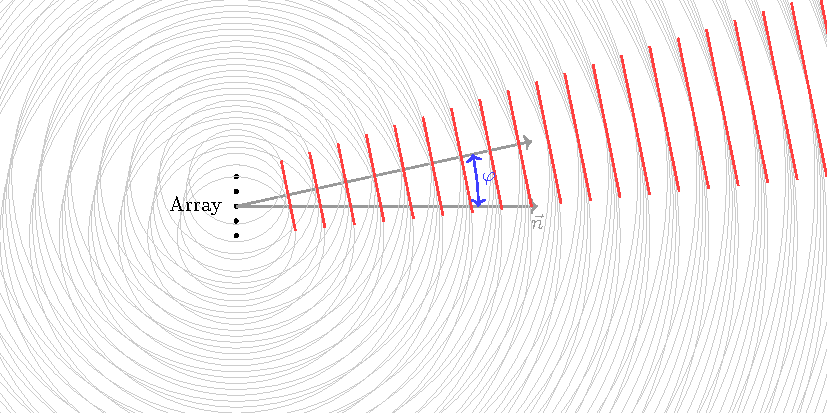
\includegraphics[]{beamforming_1.pdf}
	\caption{Phase differences between the array elements create positive interference at the red lines.
		The gray circles correspond the waves' local maxima}
	\label{ssl:fig:beamforming1}
\end{figure}

\newpage
\section{Simulator}
In order to experiment with different microphone arrangements and algorithms a simulator was developed.
Since the simulator wasn't the main focus of this Thesis, its functionality was kept simple.
The simulator lets you place acoustic sources and microphones in a $\mathbb{R}^3$ space and calculates
the measured signals at each microphone.

\subsection{Simulation Model}
For sake of simplicity the sources were modeled as omnidirectional point-sources and the
microphones are omnidirectional as well.
The Sound Pressure Level of a source is defined at one meter distance from their position and decreases
squarely with the distance.
The perceived sound at any point $P$ can now be described as
\begin{equation}
	\label[type]{ssl:eq:simcont}
	y(P, t) = \sum_{I} \frac{x_i(t - \lVert P - S_i\rVert/c)}{\lVert P - S_i\rVert}.
\end{equation}
Where $S_i$ is the position of the nth Source and $x_i(t)$ is its output sound.
Since the simulation is done numerically and with pre recorded audio files with a given
samplingrate $f_s$ \eqref{ssl:eq:simcont} has to be discretized.
Simply replacing $x_i(t - \lVert P - S_i\rVert/c)$ with
$x_i(n - f_s \lVert P - S_i\rVert/c)$ with
$n \in \mathbb{N}$ doesn't work because
$f_s \lVert P - S_i\rVert/c \not \in \mathbb{N}$ in most cases.
To implement this $f_s \lVert P - S_i\rVert/c$ is rounded to
its nearest integer $d_{P,S_i}$.
Now the delayed signal is $x_i(n - d_{P,S_i})$.
To achieve sub sample delays this signal is then filtered
with a Fractional Delay FIR Filter with a delay of
$f_s \lVert P - S_i\rVert/c - d_{P,S_i}$.


